\documentclass{beamer}
\usetheme{Warsaw}
\useinnertheme{circles}
\useoutertheme[subsection=false]{smoothbars}
\usepackage[utf8x]{inputenc}
\usepackage[czech]{babel}
\usepackage[T1]{fontenc}
\usepackage{listings}
\usepackage{tikz}
\lstset{basicstyle=\tiny\ttfamily}
\logo{
\includegraphics[height=0.5cm]{brmlab.pdf}}

\begin{document}

\AtBeginSection[]
{
  \begin{frame}
    \frametitle{Outline}
    \tableofcontents[currentsection]
  \end{frame}
}

\title{brmiversity: Umělá inteligence \\ a teoretická informatika}
\subtitle{Přednáška č. 7}
\author{Petr Baudiš $\langle${\tt pasky@ucw.cz}$\rangle$}
\institute{
	brmlab 2011\\
	\vskip 1ex
	\pgfdeclareimage[height=4ex]{ccbysa}{by-sa.pdf}
	\pgfuseimage{ccbysa}
}
\date{}
\frame{\titlepage}

\section{Umělá inteligence}

\subsection{}
\begin{frame}{Zpracování neurčité informace}
\begin{itemize}
\item Data o světě jsou neurčitá
\item Úkony ve světě jsou neurčité
\item \dots takže reálný svět je neurčitý
\item Minule jsme modelovali arbitrární vztahy mezi jevy
\item Dnes budeme modelovat {\em procesy} a {\em vstupy}
\end{itemize}
\end{frame}

\subsection{}
\begin{frame}{Markovovský řetězec}
\begin{itemize}
\item Posloupnost stavů, každý stav závisí (stochasticky) pouze na předchozím
\item $k$-tého řádu: Závislost na $k$ předchozích
\item (Je to ekvivalentní?)
\vskip 3ex
\pause
\item Velmi zjednodušený model, ale výpočetně triviální a dobrá aproximace
\vskip 3ex
\pause
\item Množina stavů, pravděpodobnosti přechodu mezi stavy
\end{itemize}

TODO ilustrace
\end{frame}

\subsection{}
\begin{frame}{Skrytý Markovovský řetězec (HMM)}
\begin{itemize}
\item {\em Skryté} stavy nedokážeme pozorovat, viditelné projevy jsou asociovány pouze přes pravděpodobnosti
\item Pravděpodobnost přechodu mezi stavy {\em a} pravděpodobnost stavu $A$ při jevu $X$
\end{itemize}

TODO ilustrace
\end{frame}

\subsection{}
\begin{frame}{Muaddib}
TODO: excerpt

\begin{itemize}
\item HMM 6. řádu --- 3 slova před, 3 slova po
\item (Začátek/konec věty: Slovo $\epsilon$)
\item TODO
\end{itemize}
\end{frame}

\subsection{}
\begin{frame}{Opakování: Normální rozdělení}
\begin{columns}
	\begin{column}{5.5cm}
		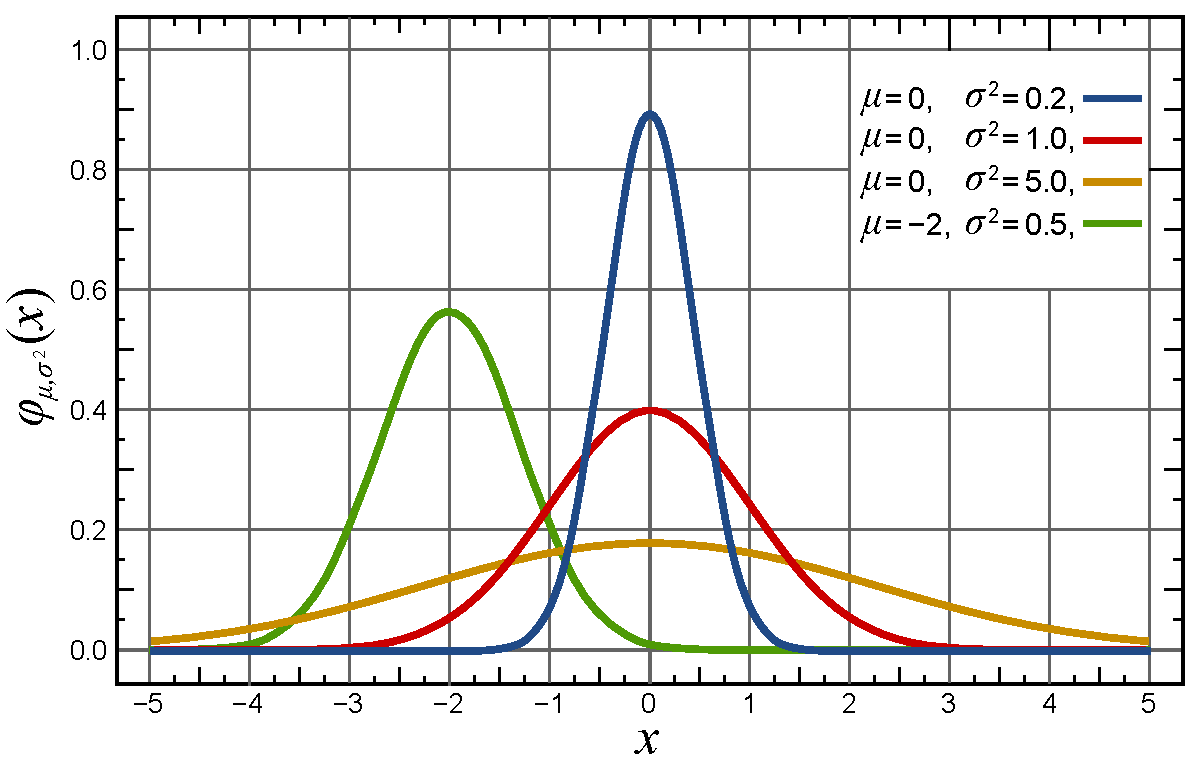
\includegraphics[width=5.5cm]{Normal_Distribution_PDF.pdf}
	\end{column}
	\begin{column}{5.5cm}
		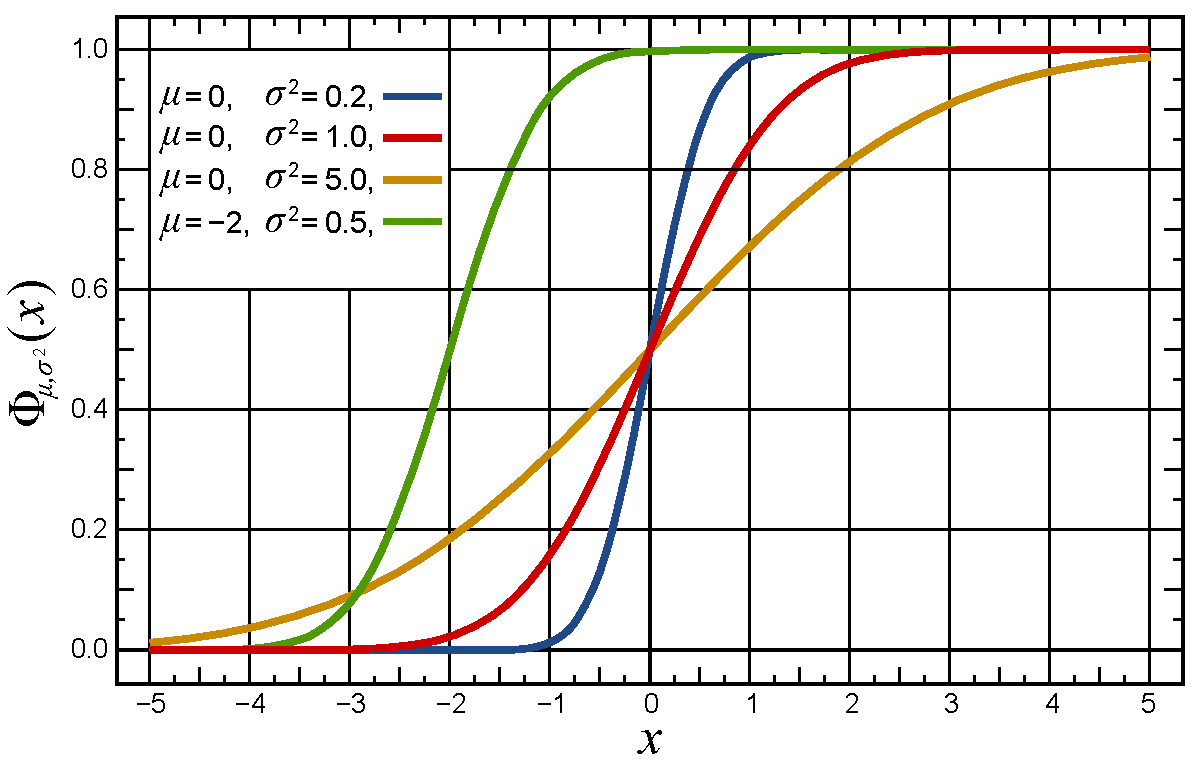
\includegraphics[width=5.5cm]{Normal_Distribution_CDF.pdf}
	\end{column}
\end{columns}

\begin{itemize}
\item {\bf Interval spolehlivosti:} S pravděpodob. $p$ bude $\mathbb{E}[X] = \mu \pm \epsilon$
\item LHC detekovalo 130 GeV ``na tři sigma''
\end{itemize}
\end{frame}

\subsection{}
\begin{frame}{Kalmánovy filtry}
\begin{itemize}
\item Svět je HMM, pozorování jsou čísla zašuměná dle normálního rozdělení
\item Různá čísla indikují (s omezenou pravděpodobností) různé stavy
\item S časem zpřesňujeme nejen odhad stavu, ale i šumu pozorování!
\end{itemize}
\end{frame}

\subsection{}
\begin{frame}{Otázky?}
\begin{center}
Příště: Strojové učení (prostor verzí, rozhodovací stromy, Bayesovské\dots)
\end{center}
\end{frame}

\section{Neuronové sítě}

\subsection{}
\begin{frame}{Data}
\begin{itemize}
\item Kovariance
\item Korelace
\item Zbytečné dimenze
\item Ilustrace
\end{itemize}
\end{frame}

\subsection{}
\begin{frame}{V-C dimenze}
\begin{itemize}
\item V-C
\item Teoretické meze
\end{itemize}
\end{frame}

\subsection{}
\begin{frame}{Principial Component Analysis}
\begin{itemize}
\item Dekolerace
\item PCA
\item Vstup --- výsledek
\item Algoritmus
\end{itemize}
\end{frame}

\subsection{}
\begin{frame}{Otázky?}
\begin{center}
Příště: Vylepšení backpropagation, struktura neuronových sítí.
\end{center}
\end{frame}

\section{Adaptivní agenti}

\subsection{}
\begin{frame}{Víceagentní systémy}
\begin{itemize}
\item Emergentní chování (``implicitní'' komunikace) \\ vs. pravidla a protokoly
\item Znalosti v multiagentních systémech
\end{itemize}
\end{frame}

\subsection{}
\begin{frame}{Komunikace v multiagentních systémech}
\begin{itemize}
\item Komunikační protokoly
\end{itemize}
\end{frame}

\subsection{}
\begin{frame}{Znalosti v multiagentních systémech}
\begin{itemize}
\item Zablácené děti
\item Modální logika
\item Dva přístupy
\item Základní věty
\end{itemize}
\end{frame}

\subsection{}
\begin{frame}{Složitější problémy distribuovaných systémů}
\begin{itemize}
\item Byzantští generálové
\item Synchronizace času
\item Ověřování událostí
\end{itemize}
\end{frame}

\subsection{}
\begin{frame}{Otázky?}
\begin{center}
Příště: Metody pro řízení agentů.
\end{center}
\end{frame}

\section{Datové struktury}

\subsection{}
\begin{frame}{Hashování}
\begin{itemize}
\item Hashovací funkce indexuje hashovací tabulku, řešíme kolize
\item Proč řešíme kolize? Vkládání a mazání (read-write struktura)
\item Perfektní a univerzální hashování
\end{itemize}
\end{frame}

\subsection{}
\begin{frame}{Perfektní hashování}
\begin{itemize}
\item Všechny klíče známe předem, vyrábíme {\em perfektní} hashovací funkci
\end{itemize}
\end{frame}

\subsection{}
\begin{frame}{Univerzální hashování}
\begin{itemize}
\item Minimalizujeme kolize i při nerovnoměrném rozdělení vstupu
\end{itemize}
\end{frame}

\subsection{}
\begin{frame}{Externí hashování}
\begin{itemize}
\item Stránky atd.
\end{itemize}
\end{frame}

\subsection{}
\begin{frame}{Otázky?}
\begin{center}
Příště: Binární vyhledávací stromy. \\ Pokročilejší druhy hald.
\end{center}
\end{frame}

\subsection{}
\begin{frame}{Děkuji vám}
\begin{center}
{\bf pasky@ucw.cz}

\vskip 6ex

Příště: Adaptivní agenti. Neuronové sítě. \\ Složitost (míry a vztahy složitosti). \\ Vyčíslitelnost (věta o rekurzi).
\end{center}
\end{frame}

\end{document}
